\documentclass[11pt]{article}

% ---------- Packages ----------
\usepackage[T1]{fontenc}
\usepackage[margin=0.95in]{geometry}
\usepackage{xcolor}
\usepackage{titlesec}
\usepackage{enumitem}
\usepackage{longtable}
\usepackage{booktabs}
\usepackage{array}
\usepackage{tabularx}
\usepackage{amsmath,amssymb}
\usepackage{tikz}
\usetikzlibrary{matrix,arrows.meta,positioning}
\usepackage[skins,breakable]{tcolorbox}
\usepackage{fancyhdr}
\usepackage{hyperref}

% ---------- Colors ----------
\definecolor{unitblue}{HTML}{1F4E79}
\definecolor{modblue}{HTML}{2E5C8A}
\definecolor{objgreen}{HTML}{2E7D32}
\definecolor{diffred}{HTML}{B71C1C}
\definecolor{prereqblue}{HTML}{0D47A1}
\definecolor{panelgray}{HTML}{F4F6F8}

% ---------- Hyperref ----------
\hypersetup{
  colorlinks=true,
  linkcolor=unitblue,
  urlcolor=unitblue,
  citecolor=unitblue,
  bookmarksopen=true,
  pdftitle={Time Series Analysis: A Complete Course Breakdown},
  pdfauthor={Course Design Document}
}

% ---------- Section styling ----------
\titleformat{\section}
  {\normalfont\Large\bfseries\color{unitblue}}
  {\thesection}{0.8em}{}[{\color{unitblue!60}\titlerule[0.8pt]}]
\titleformat{\subsection}
  {\normalfont\large\bfseries\color{modblue}}
  {\thesubsection}{0.7em}{}
\titleformat{\subsubsection}
  {\normalfont\normalsize\bfseries\color{modblue}}
  {\thesubsubsection}{0.6em}{}

\titlespacing*{\section}{0pt}{1.4em}{0.8em}
\titlespacing*{\subsection}{0pt}{1.2em}{0.5em}

% ---------- Lists ----------
\setlist[itemize]{itemsep=2pt, topsep=3pt, leftmargin=1.4em}
\setlist[itemize,2]{itemsep=1pt}

% ---------- Header/Footer ----------
\pagestyle{fancy}
\fancyhf{}
\renewcommand{\headrulewidth}{0.4pt}
\fancyhead[L]{\small\textcolor{unitblue}{Time Series Analysis --- Course Breakdown}}
\fancyhead[R]{\small\textcolor{unitblue}{\leftmark}}
\fancyfoot[C]{\small\thepage}

% ---------- Callout boxes ----------
\newtcolorbox{objectives}{
  enhanced, breakable, colback=objgreen!5, colframe=objgreen!70!black,
  boxrule=0.6pt, arc=1.5pt, left=6pt, right=6pt, top=4pt, bottom=4pt,
  fonttitle=\bfseries\small, coltitle=white, colbacktitle=objgreen!70!black,
  title={Learning Objectives}
}
\newtcolorbox{difficult}{
  enhanced, breakable, colback=diffred!5, colframe=diffred!70!black,
  boxrule=0.6pt, arc=1.5pt, left=6pt, right=6pt, top=4pt, bottom=4pt,
  fonttitle=\bfseries\small, coltitle=white, colbacktitle=diffred!70!black,
  title={Difficult Topics \& Common Pitfalls}
}
\newtcolorbox{prereqs}{
  enhanced, breakable, colback=prereqblue!5, colframe=prereqblue!70!black,
  boxrule=0.6pt, arc=1.5pt, left=6pt, right=6pt, top=4pt, bottom=4pt,
  fonttitle=\bfseries\small, coltitle=white, colbacktitle=prereqblue!70!black,
  title={Prerequisites}
}
\newtcolorbox{moduletitle}[1]{
  enhanced, colback=modblue!8, colframe=modblue,
  boxrule=0.7pt, arc=2pt, left=8pt, right=8pt, top=5pt, bottom=5pt,
  fonttitle=\bfseries, coltitle=white, colbacktitle=modblue,
  title={#1}
}

% ---------- Small helpers ----------
\newcommand{\keytopics}{\textbf{\color{modblue}Key Topics}}
\newcommand{\keyconcepts}{\textbf{\color{modblue}Key Concepts}}

\title{\color{unitblue}\textbf{Time Series Analysis}\\[4pt]\Large\textcolor{black}{A Complete Course Breakdown}}
\author{Course Design Document\\[2pt]\normalsize Based on the table of contents of\\ \emph{Time Series Analysis: With Applications in R} (Cryer \& Chan)}
\date{}

\begin{document}
\maketitle
\thispagestyle{empty}

\begin{center}
\begin{tcolorbox}[enhanced, width=0.9\textwidth, colback=panelgray, colframe=unitblue!60, arc=2pt, boxrule=0.6pt]
\small
\textbf{How to use this document.} This breakdown reorganizes the source textbook's 15 chapters and associated appendices into five instructional units and fifteen teaching modules. Each module lists its key topics, key concepts, learning objectives, difficult topics, and prerequisites, so that the material can be adopted directly as a syllabus or adapted into a one- or two-semester sequence.
\end{tcolorbox}
\end{center}

\newpage
\tableofcontents
\newpage

% ======================================================================
\section{Course Overview}
% ======================================================================

\subsection{Course Description}
This course provides a comprehensive, application-oriented treatment of the analysis and modeling of time-ordered data. Students progress from foundational probabilistic concepts, through the full iterative Box--Jenkins modeling cycle (specification, estimation, diagnostic checking, and forecasting) for stationary and nonstationary linear models, and then extend that toolkit to seasonal data, regression-based models, conditionally heteroscedastic (volatility) models, frequency-domain (spectral) methods, and nonlinear threshold models. Computation and data analysis are integrated throughout using R and its companion time-series packages.

\subsection{Course-Level Prerequisites}
\begin{itemize}
  \item \textbf{Calculus I--II:} sequences, series, limits, and basic differentiation/integration.
  \item \textbf{Probability and mathematical statistics:} expectation, variance, covariance, joint and conditional distributions, estimation theory, and hypothesis testing.
  \item \textbf{Linear regression / applied linear models:} ordinary least squares, statistical inference for regression coefficients, and residual diagnostics.
  \item \textbf{Linear algebra:} matrix operations and characteristic (eigenvalue) equations, used when analyzing stationarity and state-space representations.
  \item \textbf{Basic R programming} (or willingness to acquire it in parallel through the lab component); prior programming exposure is helpful but not required.
\end{itemize}

\subsection{Course-Level Learning Outcomes}
By the end of the course, students will be able to:
\begin{enumerate}[itemsep=3pt]
  \item Distinguish stationary from nonstationary series and select appropriate transformations or differencing strategies.
  \item Specify, estimate, diagnose, and forecast ARIMA and seasonal ARIMA models on real data using the Box--Jenkins methodology.
  \item Model interventions, outliers, and relationships between multiple time series using time-series regression techniques.
  \item Model and forecast time-varying volatility using ARCH and GARCH models.
  \item Analyze a time series in the frequency domain, including periodogram-based and smoothed spectral density estimation.
  \item Detect nonlinearity and fit threshold autoregressive models when linear models are inadequate.
  \item Communicate modeling decisions and forecast results clearly, supported by appropriate diagnostics and reproducible R code.
\end{enumerate}

\subsection{Program Structure at a Glance}
\begin{longtable}{@{}p{2.7cm}p{3.9cm}p{2.0cm}p{6.0cm}@{}}
\toprule
\textbf{Unit} & \textbf{Chapters Covered} & \textbf{Weeks} & \textbf{Theme} \\
\midrule
\endhead
Unit I & Ch.\ 1--3 & 1--3 & Foundations: examples, stochastic processes, stationarity, trend/regression \\
Unit II & Ch.\ 4--7 & 4--7 & Building the linear ARIMA toolkit: stationary and nonstationary models, specification, estimation \\
Unit III & Ch.\ 8--9 & 8--10 & Model-building capstone: diagnostics and forecasting \\
Unit IV & Ch.\ 10--12 & 11--13 & Extensions: seasonal models, time series regression, ARCH/GARCH volatility models \\
Unit V & Ch.\ 13--15 & 14--16 & Frequency domain and nonlinear models: spectral analysis and threshold models \\
\bottomrule
\end{longtable}

\subsection{Prerequisite Dependency Map}
The diagram below traces how each chapter/module depends on earlier material. Solid arrows show the primary, sequential prerequisite chain; dashed arrows highlight important cross-cutting dependencies that are easy to overlook (for example, GARCH estimation in Module 12 leans heavily on the maximum-likelihood machinery of Module 7, even though the chapters are not adjacent).

\begin{center}
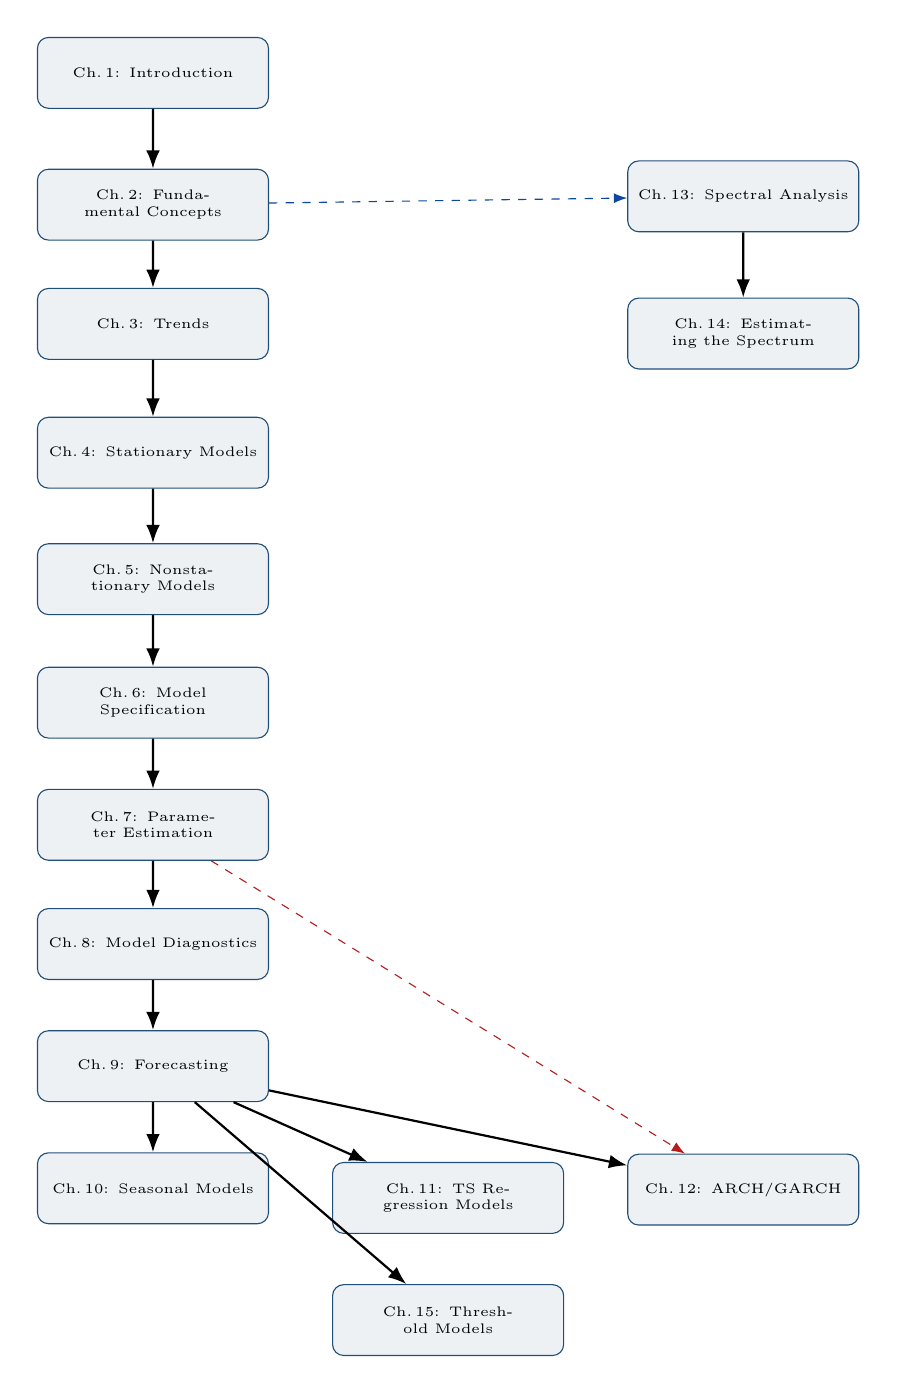
\begin{tikzpicture}[scale=0.92, every node/.style={transform shape}]
\matrix (m) [matrix of nodes,
  nodes={draw=unitblue, rounded corners, fill=unitblue!8, align=center, font=\tiny, text width=2.7cm, minimum height=0.9cm},
  row sep=6mm, column sep=8mm, nodes in empty cells] {
Ch.\,1: Introduction & |[draw=none,fill=none]| & |[draw=none,fill=none]| \\
Ch.\,2: Fundamental Concepts & |[draw=none,fill=none]| & Ch.\,13: Spectral Analysis \\
Ch.\,3: Trends & |[draw=none,fill=none]| & Ch.\,14: Estimating the Spectrum \\
Ch.\,4: Stationary Models & |[draw=none,fill=none]| & |[draw=none,fill=none]| \\
Ch.\,5: Nonstationary Models & |[draw=none,fill=none]| & |[draw=none,fill=none]| \\
Ch.\,6: Model Specification & |[draw=none,fill=none]| & |[draw=none,fill=none]| \\
Ch.\,7: Parameter Estimation & |[draw=none,fill=none]| & |[draw=none,fill=none]| \\
Ch.\,8: Model Diagnostics & |[draw=none,fill=none]| & |[draw=none,fill=none]| \\
Ch.\,9: Forecasting & |[draw=none,fill=none]| & |[draw=none,fill=none]| \\
Ch.\,10: Seasonal Models & Ch.\,11: TS Regression Models & Ch.\,12: ARCH/GARCH \\
|[draw=none,fill=none]| & Ch.\,15: Threshold Models & |[draw=none,fill=none]| \\
};
\draw[-Latex, thick] (m-1-1) -- (m-2-1);
\draw[-Latex, thick] (m-2-1) -- (m-3-1);
\draw[-Latex, thick] (m-3-1) -- (m-4-1);
\draw[-Latex, thick] (m-4-1) -- (m-5-1);
\draw[-Latex, thick] (m-5-1) -- (m-6-1);
\draw[-Latex, thick] (m-6-1) -- (m-7-1);
\draw[-Latex, thick] (m-7-1) -- (m-8-1);
\draw[-Latex, thick] (m-8-1) -- (m-9-1);
\draw[-Latex, thick] (m-9-1) -- (m-10-1);
\draw[-Latex, thick] (m-9-1) -- (m-10-2);
\draw[-Latex, thick] (m-9-1) -- (m-10-3);
\draw[-Latex, thick] (m-9-1) -- (m-11-2);
\draw[-Latex, dashed, diffred] (m-7-1) -- (m-10-3);
\draw[-Latex, dashed, prereqblue] (m-2-1) -- (m-2-3);
\draw[-Latex, thick] (m-2-3) -- (m-3-3);
\end{tikzpicture}
\end{center}
\begin{center}
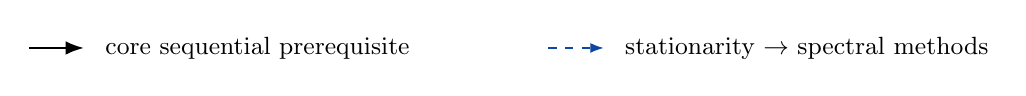
\begin{tikzpicture}[baseline]
\draw[-Latex, thick] (0,0) -- (0.7,0);
\node[anchor=west, font=\small] at (0.85,0) {core sequential prerequisite};
\draw[-Latex, dashed, prereqblue] (6.6,0) -- (7.3,0);
\node[anchor=west, font=\small] at (7.45,0) {stationarity $\rightarrow$ spectral methods};
\end{tikzpicture}\\[3pt]
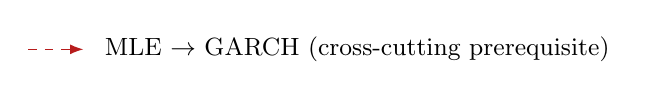
\begin{tikzpicture}[baseline]
\draw[-Latex, dashed, diffred] (0,0) -- (0.7,0);
\node[anchor=west, font=\small] at (0.85,0) {MLE $\rightarrow$ GARCH (cross-cutting prerequisite)};
\end{tikzpicture}
\end{center}

\subsection{Computational Component (R Labs)}
The source text integrates R throughout via a companion \texttt{TSA} package and a dedicated R appendix (chapter-by-chapter command reference, new/enhanced package functions, and a dataset index). This structure maps directly onto a weekly lab schedule: each module's lecture content is immediately reinforced by a hands-on lab in which students reproduce the chapter's illustrations on the provided data sets and then apply the same commands to a new series.

\subsection{Suggested Assessment Structure}
\begin{itemize}
  \item \textbf{Weekly homework / R lab exercises} tied to each module (roughly one per module).
  \item \textbf{Midterm applied project} (after Unit III): take an assigned real series through the complete Box--Jenkins cycle---specification, estimation, diagnostics, and forecasting.
  \item \textbf{Midterm examination} covering Units I--III (concepts, derivations, and interpretation).
  \item \textbf{Final project or examination} covering Units IV--V, in which students choose one extension (seasonal, regression, GARCH, spectral, or threshold analysis) and apply it to a real data set of their choosing.
\end{itemize}

\newpage
% ======================================================================
\section{Unit I: Foundations of Time Series (Weeks 1--3)}
% ======================================================================

% ---------------- Module 1 ----------------
\begin{moduletitle}{Module 1 --- Introduction to Time Series}
\small Chapter 1, pp.\ 1--10
\end{moduletitle}

\keytopics:
\begin{itemize}
  \item Real-world examples of time series drawn from economics, finance, environmental science, and engineering.
  \item The iterative Box--Jenkins model-building strategy: specification, estimation, and diagnostic checking.
  \item The historical role of time series plots in scientific and economic analysis.
  \item A roadmap of how later chapters build on one another.
\end{itemize}

\keyconcepts: time series; stochastic process (informal introduction); realization; the iterative specification--estimation--diagnostics cycle; exploratory time plots.

\begin{objectives}
\begin{itemize}
  \item Recognize and classify examples of time series data from a variety of application domains.
  \item Describe, at a conceptual level, the iterative model-building cycle used throughout the course.
  \item Explain why visual inspection of a time plot is the first step of any time series analysis.
  \item Preview how the course's chapters are organized and how each builds on the last.
\end{itemize}
\end{objectives}

\begin{difficult}
\begin{itemize}
  \item No major technical hurdles; the main conceptual shift is moving from an ``independent observations'' mindset to thinking about serially dependent data.
\end{itemize}
\end{difficult}

\begin{prereqs}
\begin{itemize}
  \item General familiarity with descriptive statistics. No time-series-specific background is required.
\end{itemize}
\end{prereqs}

\vspace{6pt}
% ---------------- Module 2 ----------------
\begin{moduletitle}{Module 2 --- Fundamental Concepts: Stochastic Processes and Stationarity}
\small Chapter 2, pp.\ 11--26
\end{moduletitle}

\keytopics:
\begin{itemize}
  \item Formal definition of a time series as a realization of a stochastic process.
  \item Mean, variance, and covariance functions of a stochastic process.
  \item The autocovariance function (ACVF) and autocorrelation function (ACF).
  \item Strict stationarity versus weak (second-order / covariance) stationarity.
  \item Appendix A: a self-contained review of expectation, variance, covariance, and correlation.
\end{itemize}

\keyconcepts: stochastic process; mean function; autocovariance function $\gamma_k$; autocorrelation function $\rho_k$; strict stationarity; weak stationarity; white noise process.

\begin{objectives}
\begin{itemize}
  \item Define a stochastic process and distinguish an observed series from the process that generated it.
  \item Compute mean, variance, and autocovariance functions for simple processes.
  \item State and apply the definitions of strict and weak stationarity.
  \item Determine whether a given process is weakly stationary from its autocovariance structure.
  \item Apply properties of expectation, variance, and covariance (Appendix A) in a time-series setting.
\end{itemize}
\end{objectives}

\begin{difficult}
\begin{itemize}
  \item Grasping that one observed series is a single realization out of infinitely many possible realizations of a stochastic process (ensemble thinking versus single-path thinking).
  \item Distinguishing strict stationarity (the entire joint distribution is time-invariant) from weak stationarity (only the first two moments are), and understanding why weak stationarity is typically sufficient in practice.
  \item Working with the general, two-argument autocovariance $\gamma(t,s)$ before it collapses to a single-argument function $\gamma_k$ under stationarity.
\end{itemize}
\end{difficult}

\begin{prereqs}
\begin{itemize}
  \item Undergraduate probability: expectation, variance, covariance, and joint distributions.
  \item Basic calculus.
\end{itemize}
\end{prereqs}

\vspace{6pt}
% ---------------- Module 3 ----------------
\begin{moduletitle}{Module 3 --- Trends and Regression Methods}
\small Chapter 3, pp.\ 27--54
\end{moduletitle}

\keytopics:
\begin{itemize}
  \item Deterministic versus stochastic trends.
  \item Estimation of a constant mean and its sampling variability.
  \item Regression-based trend estimation (linear, quadratic, seasonal-means, and harmonic/cyclical regressors).
  \item Reliability and efficiency of regression estimates when errors are autocorrelated.
  \item Interpreting standard regression output ($R^2$, $t$-tests, $F$-tests) in a time-dependent setting.
  \item Residual analysis: runs tests, residual autocorrelation, and normality checks.
\end{itemize}

\keyconcepts: deterministic trend; stochastic trend; ordinary least squares (OLS); standard-error inflation under autocorrelated errors; residual diagnostics.

\begin{objectives}
\begin{itemize}
  \item Distinguish deterministic from stochastic trends and explain why the distinction matters for modeling.
  \item Fit regression models (linear, seasonal, harmonic) to trending time series.
  \item Explain why OLS standard errors can be misleading when residuals are autocorrelated.
  \item Interpret regression output critically in a time-dependent setting.
  \item Conduct residual analysis to judge whether a fitted trend model is adequate.
\end{itemize}
\end{objectives}

\begin{difficult}
\begin{itemize}
  \item Recognizing that a high $R^2$ does not guarantee a valid time series model if the residuals are autocorrelated.
  \item Understanding how ignoring autocorrelation deflates standard errors and inflates apparent statistical significance.
  \item Distinguishing ``detrending'' from ``differencing'' as competing strategies for handling trend (a preview of a tension resolved in Module 5).
\end{itemize}
\end{difficult}

\begin{prereqs}
\begin{itemize}
  \item Introductory linear regression / simple linear model theory.
  \item Module 2 (stationarity and autocovariance), needed to interpret correlated residuals.
\end{itemize}
\end{prereqs}

\newpage
% ======================================================================
\section{Unit II: The Linear ARIMA Framework (Weeks 4--7)}
% ======================================================================

% ---------------- Module 4 ----------------
\begin{moduletitle}{Module 4 --- Models for Stationary Time Series}
\small Chapter 4, pp.\ 55--86
\end{moduletitle}

\keytopics:
\begin{itemize}
  \item The general linear process representation of a stationary series.
  \item Moving average (MA) processes: MA(1), MA($q$), and their autocorrelation structure.
  \item Autoregressive (AR) processes: AR(1), AR(2), AR($p$), and their ACF/PACF.
  \item The mixed autoregressive moving average model, ARMA($p,q$).
  \item Invertibility of moving average processes.
  \item Appendix B: the stationarity region for an AR(2) process; Appendix C: the ACF for a general ARMA($p,q$) process.
\end{itemize}

\keyconcepts: general linear process; MA($q$); AR($p$); ARMA($p,q$); characteristic equation; stationarity condition; invertibility condition; partial autocorrelation function (PACF).

\begin{objectives}
\begin{itemize}
  \item Represent a stationary process (approximately) as a general linear (infinite MA) process.
  \item Derive the ACF of MA(1) and MA($q$) processes directly from the model definition.
  \item Determine stationarity conditions for AR(1) and AR(2) processes via the characteristic equation (Appendix B).
  \item Use the PACF as the tool that distinguishes AR from MA behavior.
  \item State and interpret the invertibility condition for MA processes and explain why it is required for identifiability.
  \item Derive the ACF of a general ARMA($p,q$) model (Appendix C).
\end{itemize}
\end{objectives}

\begin{difficult}
\begin{itemize}
  \item The stationarity region for AR(2), a genuinely two-dimensional constraint on the two AR coefficients, usually visualized as a triangular admissible region.
  \item The concept of invertibility and why it is needed to resolve the non-uniqueness of MA representations.
  \item Distinguishing the theoretical ACF/PACF signatures of AR, MA, and ARMA processes from one another.
  \item Connecting complex versus real characteristic roots to damped oscillatory behavior in the ACF.
\end{itemize}
\end{difficult}

\begin{prereqs}
\begin{itemize}
  \item Module 2 (stationarity, ACVF/ACF).
  \item Difference equations and characteristic roots (typically reviewed in class).
  \item Module 3 is helpful for intuition but not strictly required.
\end{itemize}
\end{prereqs}

\vspace{6pt}
% ---------------- Module 5 ----------------
\begin{moduletitle}{Module 5 --- Models for Nonstationary Time Series: ARIMA}
\small Chapter 5, pp.\ 87--108
\end{moduletitle}

\keytopics:
\begin{itemize}
  \item Achieving stationarity through differencing.
  \item The Autoregressive Integrated Moving Average model, ARIMA($p,d,q$).
  \item The role and interpretation of constant/drift terms in ARIMA models.
  \item Variance-stabilizing and other transformations (logarithms, Box--Cox, power transformations).
  \item Appendix D: the backshift (lag) operator $B$.
\end{itemize}

\keyconcepts: differencing operator $\nabla = 1-B$; order of integration $d$; ARIMA($p,d,q$); unit root; drift term; Box--Cox transformation; backshift-operator algebra.

\begin{objectives}
\begin{itemize}
  \item Apply first- and higher-order differencing to transform a nonstationary series into a stationary one.
  \item Write and manipulate ARIMA models using backshift-operator notation (Appendix D).
  \item Explain the interpretation of a nonzero constant term in a differenced (ARIMA) model versus an undifferenced (ARMA) model.
  \item Select and apply variance-stabilizing transformations before modeling.
  \item Recognize the symptoms of underdifferencing and overdifferencing in the sample ACF.
\end{itemize}
\end{objectives}

\begin{difficult}
\begin{itemize}
  \item Overdifferencing: understanding why differencing an already-stationary series introduces spurious, hard-to-invert MA structure.
  \item Correctly interpreting the constant term in ARIMA($p,d,q$) models with $d \geq 1$ (deterministic trend versus drift in the differenced series).
  \item Operator algebra with $B$: factoring AR/MA polynomials and manipulating $\nabla^d$.
\end{itemize}
\end{difficult}

\begin{prereqs}
\begin{itemize}
  \item Module 4 (AR, MA, and ARMA models).
  \item Basic operator/polynomial algebra.
\end{itemize}
\end{prereqs}

\vspace{6pt}
% ---------------- Module 6 ----------------
\begin{moduletitle}{Module 6 --- Model Specification}
\small Chapter 6, pp.\ 109--148
\end{moduletitle}

\keytopics:
\begin{itemize}
  \item Sampling properties of the sample ACF (large-lag standard errors, Bartlett's approximation).
  \item The partial autocorrelation function (PACF) and the extended autocorrelation function (EACF).
  \item Tentative order specification using ACF/PACF/EACF patterns on simulated series.
  \item Diagnosing nonstationarity from sample ACF behavior.
  \item Other specification tools (e.g., information-criterion-based order selection).
  \item Specification case studies applied to real (``actual'') time series.
\end{itemize}

\keyconcepts: sample ACF; sample PACF; EACF table; Bartlett's formula; tentative model identification; information criteria (AIC/BIC).

\begin{objectives}
\begin{itemize}
  \item Compute and interpret sample ACF and PACF plots, including their approximate standard errors.
  \item Use the EACF table to tentatively identify the orders $(p,q)$ of an ARMA model.
  \item Distinguish stationary from nonstationary behavior in a sample ACF plot.
  \item Apply specification tools to both simulated (known-truth) and real data sets, and compare the results.
  \item Compare ACF/PACF-based specification with information-criterion-based approaches.
\end{itemize}
\end{objectives}

\begin{difficult}
\begin{itemize}
  \item Reading the EACF triangular table correctly and locating the vertex that indicates $(p,q)$.
  \item Distinguishing genuine model signatures from sampling noise in short series.
  \item Remembering that ``tentative'' specification is provisional and must be confirmed through estimation and diagnostics (Modules 7--8).
\end{itemize}
\end{difficult}

\begin{prereqs}
\begin{itemize}
  \item Modules 4--5 (ARMA/ARIMA model forms).
  \item Sampling-distribution concepts from mathematical statistics.
\end{itemize}
\end{prereqs}

\vspace{6pt}
% ---------------- Module 7 ----------------
\begin{moduletitle}{Module 7 --- Parameter Estimation}
\small Chapter 7, pp.\ 149--174
\end{moduletitle}

\keytopics:
\begin{itemize}
  \item Method-of-moments estimation (Yule--Walker equations) for AR models.
  \item Least squares estimation: conditional and unconditional (exact) sum of squares.
  \item Maximum likelihood estimation for ARMA models.
  \item Asymptotic properties of estimators: consistency, approximate normality, and standard errors.
  \item Worked illustrations of parameter estimation on real series.
  \item Bootstrapping ARIMA models for finite-sample inference.
\end{itemize}

\keyconcepts: Yule--Walker estimator; conditional sum of squares (CSS); exact/unconditional least squares; maximum likelihood estimation (MLE); asymptotic standard error; parametric bootstrap.

\begin{objectives}
\begin{itemize}
  \item Derive and compute Yule--Walker estimates for AR($p$) models.
  \item Fit ARMA/ARIMA models via conditional and unconditional least squares.
  \item Set up the likelihood function for an ARMA model and describe how it is maximized.
  \item Interpret asymptotic standard errors and construct confidence intervals for estimated coefficients.
  \item Use the bootstrap to assess estimator variability when asymptotic approximations are questionable.
\end{itemize}
\end{objectives}

\begin{difficult}
\begin{itemize}
  \item The nonlinear optimization required for exact MLE/unconditional least squares (no closed-form solution beyond the simplest AR models).
  \item Understanding how conditional least squares treats initial observations differently from exact methods, and when the difference matters.
  \item Interpreting bootstrap procedures correctly for dependent (non-i.i.d.) data.
\end{itemize}
\end{difficult}

\begin{prereqs}
\begin{itemize}
  \item Mathematical statistics: estimation theory and likelihood functions.
  \item Modules 4--6 (model forms and specification).
  \item Some exposure to numerical optimization is helpful.
\end{itemize}
\end{prereqs}

\newpage
% ======================================================================
\section{Unit III: Model-Building Capstone (Weeks 8--10)}
% ======================================================================

% ---------------- Module 8 ----------------
\begin{moduletitle}{Module 8 --- Model Diagnostics}
\small Chapter 8, pp.\ 175--190
\end{moduletitle}

\keytopics:
\begin{itemize}
  \item Residual analysis for fitted ARIMA models (standardized residuals, residual ACF).
  \item Formal portmanteau (Ljung--Box-type) tests of residual independence.
  \item Deliberate overfitting as a diagnostic strategy.
  \item Parameter redundancy: detecting unnecessarily complex fitted models.
\end{itemize}

\keyconcepts: standardized residuals; portmanteau (Ljung--Box) test; overfitting; parameter redundancy; degrees-of-freedom adjustment for estimated parameters.

\begin{objectives}
\begin{itemize}
  \item Compute and visually assess standardized residuals from a fitted ARIMA model.
  \item Apply and correctly interpret portmanteau tests for residual autocorrelation, including the degrees-of-freedom adjustment.
  \item Use deliberate overfitting to check the adequacy of a tentatively specified model.
  \item Recognize and resolve parameter redundancy in a fitted ARMA model.
\end{itemize}
\end{objectives}

\begin{difficult}
\begin{itemize}
  \item Correctly adjusting degrees of freedom in the portmanteau test to account for estimated parameters.
  \item Interpreting a ``clean'' residual ACF plot appropriately (absence of evidence is weak evidence in short series).
  \item Distinguishing genuine overfitting evidence from marginally significant, chance-driven coefficients.
\end{itemize}
\end{difficult}

\begin{prereqs}
\begin{itemize}
  \item Module 7 (estimation).
  \item Fundamentals of hypothesis testing.
\end{itemize}
\end{prereqs}

\vspace{6pt}
% ---------------- Module 9 ----------------
\begin{moduletitle}{Module 9 --- Forecasting}
\small Chapter 9, pp.\ 191--226
\end{moduletitle}

\keytopics:
\begin{itemize}
  \item The minimum mean square error (MMSE) forecasting principle.
  \item Forecasting deterministic trend models.
  \item Deriving ARIMA forecasts and their forecast error variances.
  \item Constructing prediction (forecast) limits.
  \item Worked forecasting illustrations; updating forecasts as new data arrive.
  \item Forecast weights and the connection to exponentially weighted moving averages (EWMA).
  \item Forecasting transformed series (e.g., back-transforming log-scale forecasts).
  \item Appendices E--H: conditional expectation, the proof of MMSE prediction, the truncated linear process, and an introduction to state space models.
\end{itemize}

\keyconcepts: MMSE forecast; $\ell$-step-ahead forecast; forecast error variance; prediction interval; forecast updating; EWMA; state space representation (enrichment topic).

\begin{objectives}
\begin{itemize}
  \item State and apply the MMSE forecasting principle: the optimal forecast is a conditional expectation (Appendices E--F).
  \item Derive $\ell$-step-ahead forecasts and their error variances for AR, MA, and ARMA models.
  \item Construct prediction intervals under a Gaussian assumption.
  \item Update previously computed forecasts efficiently as new observations become available.
  \item Connect simple ARIMA forecasts to exponentially weighted moving averages.
  \item Correctly forecast on the original scale when the model was fit to a transformed series.
  \item \emph{(Enrichment)} Describe how a time series model can be reformulated as a state space model (Appendix H), as a bridge to Kalman filtering.
\end{itemize}
\end{objectives}

\begin{difficult}
\begin{itemize}
  \item Formally deriving the MMSE forecast as a conditional expectation and connecting it to the truncated linear process (Appendices E--G).
  \item Computing forecast error variances that correctly account for parameter and truncation effects.
  \item Applying bias correction when back-transforming a forecast made on a transformed (e.g., logged) scale.
  \item Building intuition for the state space/Kalman filter formulation as an alternative computational framework.
\end{itemize}
\end{difficult}

\begin{prereqs}
\begin{itemize}
  \item Modules 4--7 (ARMA/ARIMA models and estimation).
  \item Conditional expectation from probability theory.
\end{itemize}
\end{prereqs}

\vspace{10pt}
\begin{tcolorbox}[enhanced, colback=panelgray, colframe=unitblue!60, arc=2pt, boxrule=0.6pt, title={Checkpoint: Midterm Applied Project}, coltitle=white, colbacktitle=unitblue, fonttitle=\bfseries]
\small After Module 9, students complete an applied project that carries a single real data set through the full Box--Jenkins cycle: exploratory plotting, transformation and differencing, tentative specification, estimation, diagnostic checking, and forecasting with prediction limits. This project consolidates Units I--III before the course moves on to specialized extensions.
\end{tcolorbox}

\newpage
% ======================================================================
\section{Unit IV: Extensions of the ARIMA Framework (Weeks 11--13)}
% ======================================================================

% ---------------- Module 10 ----------------
\begin{moduletitle}{Module 10 --- Seasonal Models}
\small Chapter 10, pp.\ 227--248
\end{moduletitle}

\keytopics:
\begin{itemize}
  \item Seasonal ARIMA (SARIMA) model formulation.
  \item Multiplicative seasonal ARMA models.
  \item Nonstationary seasonal ARIMA models and seasonal differencing.
  \item Specification, fitting, and diagnostic checking of seasonal models.
  \item Forecasting with seasonal models.
\end{itemize}

\keyconcepts: seasonal period $s$; seasonal differencing $\nabla_s$; multiplicative SARIMA$(p,d,q)\times(P,D,Q)_s$ notation; seasonal and non-seasonal polynomial factors.

\begin{objectives}
\begin{itemize}
  \item Recognize seasonal patterns in the ACF/PACF at multiples of the seasonal period.
  \item Specify a multiplicative SARIMA model appropriate to a given seasonal series.
  \item Apply seasonal and combined seasonal/regular differencing to induce stationarity.
  \item Fit, diagnose, and forecast seasonal ARIMA models on real seasonal data.
\end{itemize}
\end{objectives}

\begin{difficult}
\begin{itemize}
  \item Interpreting the multiplicative structure (a product of seasonal and non-seasonal polynomials) and what it implies for the ACF.
  \item Deciding between seasonal differencing and seasonal dummy/harmonic regressors (a callback to Module 3).
  \item Avoiding overdifferencing when both regular and seasonal differencing are applied.
\end{itemize}
\end{difficult}

\begin{prereqs}
\begin{itemize}
  \item Modules 4--9 (the full linear ARIMA modeling cycle).
  \item Module 3 (deterministic seasonal regressors, for comparison).
\end{itemize}
\end{prereqs}

\vspace{6pt}
% ---------------- Module 11 ----------------
\begin{moduletitle}{Module 11 --- Time Series Regression Models}
\small Chapter 11, pp.\ 249--276
\end{moduletitle}

\keytopics:
\begin{itemize}
  \item Intervention analysis: modeling the effect of a known event or policy change.
  \item Detecting and modeling outliers (additive and innovational).
  \item Spurious correlation between nonstationary or trending series.
  \item Prewhitening and stochastic regression for relating two time series.
\end{itemize}

\keyconcepts: intervention/transfer function model; additive outlier (AO); innovational outlier (IO); spurious regression; cross-correlation function (CCF); prewhitening.

\begin{objectives}
\begin{itemize}
  \item Build intervention models that quantify the effect of a discrete event on a time series.
  \item Identify and appropriately model additive versus innovational outliers.
  \item Explain why regressing one trending or nonstationary series on another can produce spuriously significant results.
  \item Apply prewhitening to correctly assess the relationship between two time series.
\end{itemize}
\end{objectives}

\begin{difficult}
\begin{itemize}
  \item Distinguishing additive from innovational outliers and choosing the correct intervention indicator and timing.
  \item Understanding the mechanism behind spurious correlation in nonstationary series and why classical regression assumptions fail.
  \item Correctly executing and interpreting the prewhitening procedure.
\end{itemize}
\end{difficult}

\begin{prereqs}
\begin{itemize}
  \item Module 3 (regression).
  \item Modules 4--9 (ARIMA modeling, residual diagnostics used in outlier detection).
\end{itemize}
\end{prereqs}

\vspace{6pt}
% ---------------- Module 12 ----------------
\begin{moduletitle}{Module 12 --- Time Series Models of Heteroscedasticity: ARCH/GARCH}
\small Chapter 12, pp.\ 277--318
\end{moduletitle}

\keytopics:
\begin{itemize}
  \item Stylized facts of financial time series (volatility clustering, heavy tails, near-zero return autocorrelation).
  \item The ARCH(1) model.
  \item GARCH($p,q$) models.
  \item Maximum likelihood estimation for ARCH/GARCH models.
  \item Model diagnostics for volatility models.
  \item Conditions ensuring nonnegativity of the conditional variance.
  \item Extensions of the GARCH model; applied example using daily USD/HKD exchange rates.
  \item Appendix I: formulas for generalized portmanteau tests applied to squared residuals.
\end{itemize}

\keyconcepts: conditional heteroscedasticity; volatility clustering; ARCH(1); GARCH($p,q$); conditional variance equation; nonnegativity constraints; leverage effect.

\begin{objectives}
\begin{itemize}
  \item Identify stylized facts of financial return series that motivate ARCH/GARCH modeling.
  \item Specify and estimate ARCH(1) and GARCH($p,q$) models via maximum likelihood.
  \item Diagnose the adequacy of a fitted volatility model (e.g., via squared standardized residuals).
  \item State the coefficient conditions that guarantee a nonnegative conditional variance.
  \item Compare basic GARCH with an asymmetric/extended variant and explain the motivation for the extension.
\end{itemize}
\end{objectives}

\begin{difficult}
\begin{itemize}
  \item Setting up and numerically maximizing the (often non-Gaussian) likelihood function for GARCH models.
  \item Reasoning about nonnegativity and stationarity (finite unconditional variance) conditions simultaneously.
  \item Distinguishing conditional from unconditional heteroscedasticity, and volatility modeling from mean modeling.
\end{itemize}
\end{difficult}

\begin{prereqs}
\begin{itemize}
  \item Module 7 (maximum likelihood estimation) --- the single most important prerequisite for this module.
  \item Module 2 (stationarity).
  \item Basic exposure to financial returns is helpful but not required.
\end{itemize}
\end{prereqs}

\newpage
% ======================================================================
\section{Unit V: Frequency Domain and Nonlinear Models (Weeks 14--16)}
% ======================================================================

% ---------------- Module 13 ----------------
\begin{moduletitle}{Module 13 --- Introduction to Spectral Analysis}
\small Chapter 13, pp.\ 319--350
\end{moduletitle}

\keytopics:
\begin{itemize}
  \item Motivation for a frequency-domain view of time series.
  \item The periodogram as an empirical frequency-domain summary.
  \item The spectral representation and spectral distribution function.
  \item The spectral density function and its relationship to the ACVF.
  \item Spectral densities of ARMA processes.
  \item Sampling properties of the sample spectral density.
  \item Appendix J: orthogonality of cosine and sine sequences.
\end{itemize}

\keyconcepts: frequency domain; periodogram; spectral distribution function; spectral density $f(\omega)$; Fourier transform pair with the ACVF; orthogonality of trigonometric sequences.

\begin{objectives}
\begin{itemize}
  \item Explain, at a conceptual level, how a stationary process can be decomposed into contributions from different frequencies.
  \item Compute and interpret the periodogram of a time series.
  \item Derive the spectral density of simple AR/MA/ARMA processes from their ACVF.
  \item Describe the sampling distribution of periodogram ordinates and explain why the raw periodogram is an inconsistent estimator of the spectral density.
\end{itemize}
\end{objectives}

\begin{difficult}
\begin{itemize}
  \item Moving from an intuitive to a rigorous understanding of the spectral representation theorem.
  \item Working comfortably with complex exponentials and trigonometric identities (Appendix J).
  \item Understanding why periodogram ordinates are asymptotically independent and exponentially distributed, yet remain inconsistent estimators of the spectral density.
\end{itemize}
\end{difficult}

\begin{prereqs}
\begin{itemize}
  \item Module 2 (ACVF, stationarity).
  \item Complex numbers and basic Fourier series (often reviewed in class).
\end{itemize}
\end{prereqs}

\vspace{6pt}
% ---------------- Module 14 ----------------
\begin{moduletitle}{Module 14 --- Estimating the Spectrum}
\small Chapter 14, pp.\ 351--382
\end{moduletitle}

\keytopics:
\begin{itemize}
  \item Smoothing the periodogram to estimate the spectral density.
  \item The bias--variance tradeoff in spectral smoothing.
  \item Bandwidth selection.
  \item Confidence intervals for the spectrum.
  \item Leakage and tapering.
  \item Autoregressive (parametric) spectrum estimation.
  \item Appendix K: tapering and the Dirichlet kernel.
\end{itemize}

\keyconcepts: smoothed periodogram; spectral window; bandwidth; leakage; tapering; Dirichlet kernel; AR-based spectral estimation.

\begin{objectives}
\begin{itemize}
  \item Apply smoothing techniques to obtain a consistent spectral density estimate.
  \item Explain the bias--variance tradeoff governing bandwidth choice and select a reasonable bandwidth.
  \item Construct approximate confidence intervals for a smoothed spectral estimate.
  \item Explain the leakage phenomenon and apply tapering to mitigate it.
  \item Estimate the spectral density parametrically via a fitted AR model and compare it with nonparametric estimates.
\end{itemize}
\end{objectives}

\begin{difficult}
\begin{itemize}
  \item Choosing an appropriate bandwidth in practice: the fundamental nonparametric bias--variance tradeoff.
  \item Understanding leakage as a consequence of finite-sample truncation, and the role of the Dirichlet kernel in explaining it (Appendix K).
  \item Reconciling parametric (AR-based) and nonparametric spectral estimates that disagree.
\end{itemize}
\end{difficult}

\begin{prereqs}
\begin{itemize}
  \item Module 13 (periodogram, spectral density).
  \item Comfort with Fourier-type reasoning.
\end{itemize}
\end{prereqs}

\vspace{6pt}
% ---------------- Module 15 ----------------
\begin{moduletitle}{Module 15 --- Threshold (Nonlinear) Models}
\small Chapter 15, pp.\ 383--421
\end{moduletitle}

\keytopics:
\begin{itemize}
  \item Graphical tools for exploring nonlinearity in time series.
  \item Formal tests for nonlinearity.
  \item Why simple polynomial nonlinear extensions of AR models tend to be dynamically explosive.
  \item First-order threshold autoregressive (TAR) models.
  \item General (multi-regime) threshold models.
  \item Testing for threshold-type nonlinearity.
  \item Estimating a TAR model, including its threshold and delay parameters.
  \item Model diagnostics and prediction for TAR models.
  \item Appendix L: a generalized portmanteau test for TAR models.
\end{itemize}

\keyconcepts: nonlinearity; regime switching; threshold autoregressive (TAR) model; self-exciting TAR (SETAR); threshold-parameter estimation.

\begin{objectives}
\begin{itemize}
  \item Use graphical diagnostics and formal tests to detect nonlinearity that a linear ARMA model cannot capture.
  \item Explain why naive polynomial extensions of AR models are typically dynamically unstable.
  \item Specify and estimate a self-exciting threshold autoregressive model, including its delay and threshold parameters.
  \item Perform diagnostic checking and generate forecasts from a fitted TAR model.
  \item Compare a fitted TAR model against its best-fitting linear ARIMA competitor.
\end{itemize}
\end{objectives}

\begin{difficult}
\begin{itemize}
  \item Estimating the threshold parameter, which typically requires a grid search over a non-smooth objective rather than standard likelihood methods.
  \item Non-standard asymptotic theory for tests of threshold nonlinearity (test statistics do not follow standard distributions under the null hypothesis).
  \item Multi-step forecasting from a nonlinear model, which generally has no closed-form MMSE solution and often requires simulation.
\end{itemize}
\end{difficult}

\begin{prereqs}
\begin{itemize}
  \item Modules 4--9 (the full linear ARIMA toolkit, used as the baseline/competitor model).
  \item Module 7 (estimation), extended here to non-smooth optimization problems.
\end{itemize}
\end{prereqs}

\newpage
% ======================================================================
\section{Cross-Cutting Difficult Topics}
% ======================================================================
The table below collects the concepts that, across many offerings of this material, most often need a second pass, together with a quick teaching tip for each.

\begin{longtable}{@{}p{4.3cm}p{1.6cm}p{7.3cm}@{}}
\toprule
\textbf{Concept} & \textbf{Module} & \textbf{Teaching Tip} \\
\midrule
\endhead
Strict vs.\ weak stationarity & 2 & Simulate many realizations of the same process to make the ``ensemble'' idea concrete before collapsing to one observed path. \\
AR(2) stationarity region / characteristic roots & 4 & Plot the triangular admissible region in the $(\phi_1,\phi_2)$ plane and place example models on it. \\
Invertibility of MA models & 4 & Show two MA(1) models with reciprocal roots that produce identical ACFs, motivating the invertibility restriction. \\
MMSE forecasting via conditional expectation & 9 & Work a fully explicit AR(1) forecast by hand, step by step, before generalizing. \\
GARCH likelihood optimization \& nonnegativity & 12 & Visualize simulated conditional-variance paths under parameter choices that satisfy, and violate, the nonnegativity conditions. \\
Spectral representation theorem & 13 & Connect explicitly back to the Fourier series students already know from calculus/signals courses. \\
Bandwidth selection in spectral smoothing & 14 & Run an interactive bias--variance demonstration, varying the bandwidth on the same series. \\
Threshold-parameter estimation & 15 & Plot the sum of squared residuals against candidate threshold values to make the grid search visible. \\
\bottomrule
\end{longtable}

\newpage
% ======================================================================
\section{Suggested 16-Week Schedule}
% ======================================================================
\begin{longtable}{@{}p{1.1cm}p{4.6cm}p{5.4cm}p{2.7cm}@{}}
\toprule
\textbf{Week} & \textbf{Module (Chapter)} & \textbf{Focus} & \textbf{Deliverable} \\
\midrule
\endhead
1 & Module 1 (Ch.\ 1) & Introduction to time series & Lab 0: R \& \texttt{TSA} setup \\
2 & Module 2 (Ch.\ 2) & Stochastic processes, stationarity & HW 1 \\
3 & Module 3 (Ch.\ 3) & Trends and regression & HW 2, Lab 1 \\
4 & Module 4 (Ch.\ 4), part 1 & MA and AR processes & HW 3 \\
5 & Module 4 (Ch.\ 4), part 2 & ARMA, invertibility & Lab 2 \\
6 & Module 5 (Ch.\ 5) & ARIMA, differencing & HW 4 \\
7 & Module 6 (Ch.\ 6) & Model specification & Lab 3, HW 5 \\
8 & Module 7 (Ch.\ 7) & Parameter estimation & Midterm exam (Units I--II) \\
9 & Module 8 (Ch.\ 8) & Model diagnostics & Lab 4 \\
10 & Module 9 (Ch.\ 9) & Forecasting & Midterm applied project due \\
11 & Module 10 (Ch.\ 10) & Seasonal models & HW 6 \\
12 & Module 11 (Ch.\ 11) & Intervention, outliers, prewhitening & Lab 5 \\
13 & Module 12 (Ch.\ 12) & ARCH/GARCH & HW 7 \\
14 & Module 13 (Ch.\ 13) & Spectral analysis: periodogram \& spectral density & Lab 6 \\
15 & Modules 14--15 (Ch.\ 14--15) & Estimating the spectrum; threshold models (survey) & HW 8 \\
16 & Review & Synthesis and integration & Final project presentations / final exam \\
\bottomrule
\end{longtable}

\newpage
% ======================================================================
\section{Final Notes for Instructors}
% ======================================================================
\begin{itemize}
  \item \textbf{One semester vs.\ two.} The 16-week schedule above is intentionally dense in its final third. Programs that prefer a gentler pace can split the material into a two-course sequence: \emph{Time Series Analysis I} covering Units I--III (Chapters 1--9, the complete linear Box--Jenkins cycle), and \emph{Time Series Analysis II} covering Units IV--V (Chapters 10--15, the specialized extensions), with the latter treated as an advanced/elective course.
  \item \textbf{Mathematical appendices as enrichment.} Several appendices in the source text (B, C, D, E--H, I, J, K, L) contain the technical derivations underlying each chapter's results. They are listed under the relevant module above and can be assigned as core reading for a more theoretical, graduate-level offering, or left as optional enrichment for a more applied offering.
  \item \textbf{Computation is not an add-on.} Because every chapter of the source material has a matching R-commands section and the companion \texttt{TSA} package supplies the illustrative data sets, the lab sequence in Section~1.6 should run in lockstep with lecture, not trail behind it.
  \item \textbf{Capstone flexibility.} The Unit III midterm project and the Unit IV--V final project are both designed to be satisfied with a data set of the student's choosing, which keeps the course's heavy methodological load anchored to a single, increasingly familiar application throughout the term.
\end{itemize}

\end{document}